\chapter{Problem 1 - Arsitektur \& Interoperabilitas Data}

\section{Rancangan Solusi}

Menggunakan REST sebagai metode komunikasi antara BNPB dengan BMKG/PVMBG. Kontrak GET API BMKG akan terlihat berikut ini:\\
GET /seismic-events?since=\textless timestamp\textgreater{}

\begin{codebox}
{
    "event_id": <string_value>,
    "magnitude": <float_value>,
    "depth_km": <float_value>,
    "epicenter_lat": <float_value>,
    "epicenter_lon": <float_value>,
    "region_name": <string_value>,
    "occurred_at": <datetime_value_in_string>,
    "potential_tsunami": <boolean_value>,
}
\end{codebox}

GET /tsunami-warnings?since=\textless timestamp\textgreater{}

\begin{codebox}
{
    "warning_id": <string_value>,
    "related_event_id": <string_value>,
    "threat_level": <enum_value_in_string>,
    "affected_zones":
    [
        <string_value>,
        <string_value>,
    ],
    "estimated_arrival": <date_time>,
}
\end{codebox}

Sedangkan, Kontrak GET API PVMBG akan terlihat seperti berikut ini:\\
GET /volcanic-reports?since=\textless timestamp\textgreater{}

\begin{codebox}
{
    "report_id": <string_value>,
    "volcano_id": <string_value>,
    "alert_level": <enum_value_in_string>,
    "eruption_count_24h": <integer_value>,
    "ash_column_height_m": <float_value>,
    "reported_at": <datetime_value>,
}
\end{codebox}

Kontrak API di atas merupakan yang terdefinisikan dalam BNPB dan bagaimana cara BNPB memetakan nilainya sesuai dengan \href{https://docs.google.com/document/d/1QOSgL0U4eBN-16b3Hkr7ohzDLYPmPC0tlI-CoFZSRm8/edit?tab=t.0\#heading=h.ql4pp1hq9xtx}{spesifikasi tugas besar}. Untuk seluruh \emph{field} yang belum didefinisikan tapi muncul dalam JSON yang dikembalikan, BNPB akan memetakan field baru tersebut ke dalam field \emph{attributes}. Untuk seluruh \emph{fields} yang sudah didefinisikan tapi tidak ada dalam JSON yang dikembalikan, field terkait bernilai \emph{null}. Untuk seluruh field yang di-\emph{rename}, mekanisme sebelumnya (field removal dan field addition) akan secara otomatis menangani masalah ini. Untuk tipe data yang diubah, field terkait akan dimasukkan ke \emph{attribute field} dengan nama key yang sama.

\subsection{Format Kanonik HazardEvent}

Aggregator memetakan setiap rekaman dari kedua sumber ke \texttt{HazardEvent}. Sepuluh field pertama disimpan sebagai kolom bertipe, dan \texttt{attributes} menampung sisanya sebagai JSONB.

\begin{longtable}[]{|>{\raggedright\arraybackslash}p{0.22\linewidth}|>{\raggedright\arraybackslash}p{0.2\linewidth}|>{\raggedright\arraybackslash}p{0.2\linewidth}|>{\raggedright\arraybackslash}p{0.3\linewidth}|}
\hline
Field & Tipe & Klasifikasi & Keterangan \\
\hline
\endhead
\texttt{hazard\_id} & UUID & Ringkasan & Dibangkitkan Aggregator \\
\hline
\texttt{source} & BMKG atau PVMBG & Ringkasan & Instansi asal \\
\hline
\texttt{source\_ref\_id} & string & Mentah & Identifier asli di sumber \\
\hline
\texttt{hazard\_type} & SEISMIC atau VOLCANIC & Ringkasan & Konstan per sumber \\
\hline
\texttt{severity} & NORMAL, WASPADA, SIAGA, AWAS & Ringkasan & Boleh \textit{null} \\
\hline
\texttt{area\_name} & string & Ringkasan & Boleh \textit{null} \\
\hline
\texttt{latitude}, \texttt{longitude} & float & Mentah & Boleh \textit{null} \\
\hline
\texttt{occurred\_at} & datetime & Ringkasan & Waktu kejadian \\
\hline
\texttt{ingested\_at} & datetime & Ringkasan & Waktu Aggregator menerima \\
\hline
\texttt{attributes} & JSONB & Mentah & Field sumber tanpa padanan kanonik \\
\hline
\end{longtable}

\subsection{Aturan Pemetaan}

\begin{longtable}[]{|>{\raggedright\arraybackslash}p{0.22\linewidth}|>{\raggedright\arraybackslash}p{0.34\linewidth}|>{\raggedright\arraybackslash}p{0.34\linewidth}|}
\hline
Kanonik & SeismicEvent (BMKG) & VolcanicReport (PVMBG) \\
\hline
\endhead
\texttt{source\_ref\_id} & \texttt{event\_id} & \texttt{report\_id} \\
\hline
\texttt{hazard\_type} & SEISMIC & VOLCANIC \\
\hline
\texttt{area\_name} & \texttt{region\_name} & Nama gunung dari tabel referensi berdasarkan \texttt{volcano\_id} \\
\hline
\texttt{latitude}, \texttt{longitude} & \texttt{epicenter\_lat}, \texttt{epicenter\_lon} & Koordinat gunung dari tabel referensi \\
\hline
\texttt{occurred\_at} & \texttt{occurred\_at} & \texttt{reported\_at} \\
\hline
\texttt{severity} & Lihat aturan di bawah & \texttt{alert\_level} dipetakan langsung \\
\hline
\texttt{attributes} & \texttt{magnitude}, \texttt{depth\_km}, \texttt{potential\_tsunami}, dan \texttt{tsunami\_warning} bila ada & \texttt{eruption\_count\_24h}, \texttt{ash\_column\_height\_m}, \texttt{confidence\_level} bila ada \\
\hline
\end{longtable}

Severity gempa ditentukan berurutan. Pertama, bila ada \texttt{TsunamiWarning} yang berkorelasi lewat \texttt{related\_event\_id}, dipakai \texttt{threat\_level} dari warning paling parah (Awas menjadi AWAS). Kedua, bila tidak ada warning, dipakai magnitudo: di bawah 5,0 menjadi NORMAL, 5,0 sampai di bawah 6,5 menjadi WASPADA, dan 6,5 ke atas menjadi SIAGA. Korelasi dengan warning dilakukan di Aggregator karena BMKG hanya mengembalikan kedua daftar secara terpisah. Tabel referensi gunung api milik Aggregator berisi delapan gunung yang dipakai \textit{mock} PVMBG, karena PVMBG hanya mengirim \texttt{volcano\_id}.

Aggregator mengirim \texttt{?since=} berisi kursor dari siklus polling sebelumnya, sehingga setiap siklus hanya mengambil rekaman baru. Pemetaan bekerja pada \textit{map} generik, bukan \textit{struct} tetap, sehingga field yang tidak dikenal tetap terbawa. Setiap field yang tidak dikenal, hilang, atau berubah tipe dicatat sekali di \textit{log} beserta keputusan pemetaannya.

\section{Alasan Keputusan}

Pertama, kebijakan penanganan yang didefinisikan seperti demikian. Kedua, tertulis bahwa penambahan field baru oleh PVMBG adalah perubahan internal mereka sendiri, bukan urusan BNPB. Bagaimana cara PVMBG mengembalikan struktur JSON itu terserah PVMBG, tidak ada perjanjian yang dibuat antara BNPB dengan PVMBG. Dengan itu, BNPB harus bisa secara fleksibel support sudden schema change dari kedua BMKG dan PVMBG. Opsi lain seperti gRPC mendukung atribut yang fleksibel. Contohnya menggunakan gRPC, \emph{message} dapat didefinisikan agar mensimulasikan JSON (Paani, 2023):

\begin{codebox}
message Person
{
   string name = 1;
   int32 age = 2;
   google.protobuf.Struct additionalInfo = 3;

}
\end{codebox}

Atau menggunakan map string string dalam Thrift (roger, 2015):

\begin{codebox}
struct QuerySetRecord {
    ...
    4:map<string,string> dataMap,
    ...
}
\end{codebox}

Sedangkan GraphQL tidak support dynamic fields. Pendefinisian skema \emph{dynamic field} tersebut bisa dipakai jika PVMBG dan BMKG peduli terhadap urusan BNPB. Semisal pakai gRPC, ada dua pendekatan:

\begin{enumerate}
\def\labelenumi{\arabic{enumi}.}
\tightlist
\item
  Tambah message yang support \emph{dynamic field} dalam protobuf, sehingga field baru dimasukkan masing-masing oleh PVMBG dan BMKG ke dalam field dinamis tersebut sebelum dikembalikan ke BNPB. Pendekatan ini sama sekali tidak merepresentasikan yang ditulis oleh spek. PVMBG tidak peduli bagaimana cara skema mereka di-\emph{parse} oleh server luar. Pasti mereka akan prioritaskan kebutuhan internal mereka (tanpa menggunakan field dinamis sama sekali dalam skema protobuf).\\
\item
  Skema dari PVMBG atau BMKG diubah secara internal. Pendekatan ini tidak mendukung kebijakan yang sudah didefinisikan, karena walaupun BNPB masih bisa parse tanpa error, field yang baru ditambahkan itu tidak akan berhasil di-\emph{parse} (skema internal BNPB belum berubah, sebelum field baru ditambahkan). Belum lagi kalau urutan skema dalam sebuah message berbeda.
\end{enumerate}

Untuk thrift, pendekatannya sama seperti penjelasan di atas. Dengan demikian, pendekatan REST JSON yang fleksibel merupakan pilihan yang tepat untuk \emph{problem set} 1. REST JSON tidak memerlukan field tersendiri khusus field dinamis, dan masih dapat di-\emph{parse} secara utuh oleh BNPB-nya.


Alternatif pada tingkat mekanisme pemetaan adalah sebagai berikut.

\begin{longtable}[]{|>{\raggedright\arraybackslash}p{0.22\linewidth}|>{\raggedright\arraybackslash}p{0.4\linewidth}|>{\raggedright\arraybackslash}p{0.28\linewidth}|}
\hline
Mekanisme & Konsekuensi & Hasil \\
\hline
\endhead
\textit{Dynamic field mapping} & Field tak dikenal masuk ke \texttt{attributes} tanpa kontrak baru. Field kanonik yang bergantung pada nama atau tipe lama menjadi \textit{null}. & Dipilih \\
\hline
\textit{Schema registry} & Menuntut sumber mendaftarkan skema sebelum mengubahnya, padahal PVMBG mengubah skema tanpa memberi tahu. & Ditolak \\
\hline
Evolusi skema Protobuf atau Avro & Menuntut sumber memakai format yang sama, bertentangan dengan kontrak REST JSON dari spesifikasi. & Ditolak \\
\hline
JSON \textit{additive-only} & Menolak atau mengabaikan rename dan perubahan tipe, sehingga data tetap hilang diam-diam. & Ditolak \\
\hline
\end{longtable}

\section{Batasan Yang Disadari}

Pendekatan ini mendukung berbagai macam perubahan yang terjadi dalam skema API nya:

\begin{enumerate}
\def\labelenumi{\arabic{enumi}.}
\tightlist
\item
  Penambahan field baru: dimasukkan ke dalam field attribute.\\
\item
  Pengurangan field: nilai field terkait menjadi null.\\
\item
  Perubahan nama field: dimasukkan ke dalam field attribute, dan field terkait nama sebelumnya bernilai \emph{null}.\\
\item
  Perubahan tipe data: dimasukkan ke dalam field attribute dengan key yang sama.
\end{enumerate}

Batasan lain yang disadari:

\begin{itemize}
\tightlist
\item
  Field kanonik yang bergantung pada nama atau tipe lama menjadi \textit{null} bila field itu berubah. Misalnya bila \texttt{magnitude} berganti nama, severity cadangan kosong, dan bila \texttt{epicenter\_lat} berubah, \texttt{latitude} kosong. Nilai aslinya tetap ada di \texttt{attributes}, tetapi tidak ada komponen yang membacanya.
\item
  Rekaman dengan field identifier atau waktu yang berubah ditolak dan dihitung sebagai ditolak, karena keduanya wajib untuk menyimpan. Rekaman dengan waktu jauh di masa depan atau identifier terlalu panjang juga ditolak. Rekaman yang ditolak tidak menggagalkan siklus polling.
\item
  Perubahan makna pada field yang nama dan tipenya tetap tidak terdeteksi.
\item
  Tabel gunung api bersifat statis. \texttt{volcano\_id} baru tetap disimpan tetapi tanpa nama dan koordinat sampai tabel diubah.
\item
  Satu severity terpadu diturunkan dari skala tiap sumber, sehingga nuansa khusus sumber hanya ada di \texttt{attributes}.
\end{itemize}

\section{Kebijakan Penanganan Field Tak Dikenal}

Kebijakan yang dideklarasikan adalah semua field dari sumber yang belum memiliki padanan kanonik diteruskan ke \texttt{attributes} dengan key yang sama, dan tidak ada yang diabaikan. Field kanonik yang tidak ditemukan pada rekaman bernilai \textit{null}. Sistem berperilaku sesuai kebijakan ini, dan konsistensinya diperiksa pada Bukti Penyelesaian.

\section{Mekanisme yang Dipilih}

Mekanisme yang dipilih adalah \textit{dynamic field mapping}. Perubahan skema yang didukung, seluruhnya tanpa restart atau \textit{redeploy} Aggregator, adalah penambahan field, penghapusan field, perubahan nama field, dan perubahan tipe data. Perubahan yang secara sadar tidak didukung adalah:

\begin{itemize}
\tightlist
\item
  perubahan struktur \textit{endpoint}, yaitu path atau method, karena kontrak ditetapkan spesifikasi dan tidak boleh diubah;
\item
  perubahan makna pada field yang nama dan tipenya tetap, misalnya satuan atau skala, karena tidak ada cara mendeteksinya tanpa kontrak semantik dari sumber.
\end{itemize}

\section{Bukti Penyelesaian}

\subsection{Aggregator Menghasilkan HazardEvent}

Skenario \texttt{tests/scenarios/problem1.sh} menampilkan hasil pemetaan dari PVMBG pada skema awal. Tiga laporan vulkanik terbaru belum membawa \texttt{confidence\_level}, sedangkan \texttt{severity} dan \texttt{area\_name} sudah terisi dari aturan pemetaan.

\begin{figure}[H]
\centering
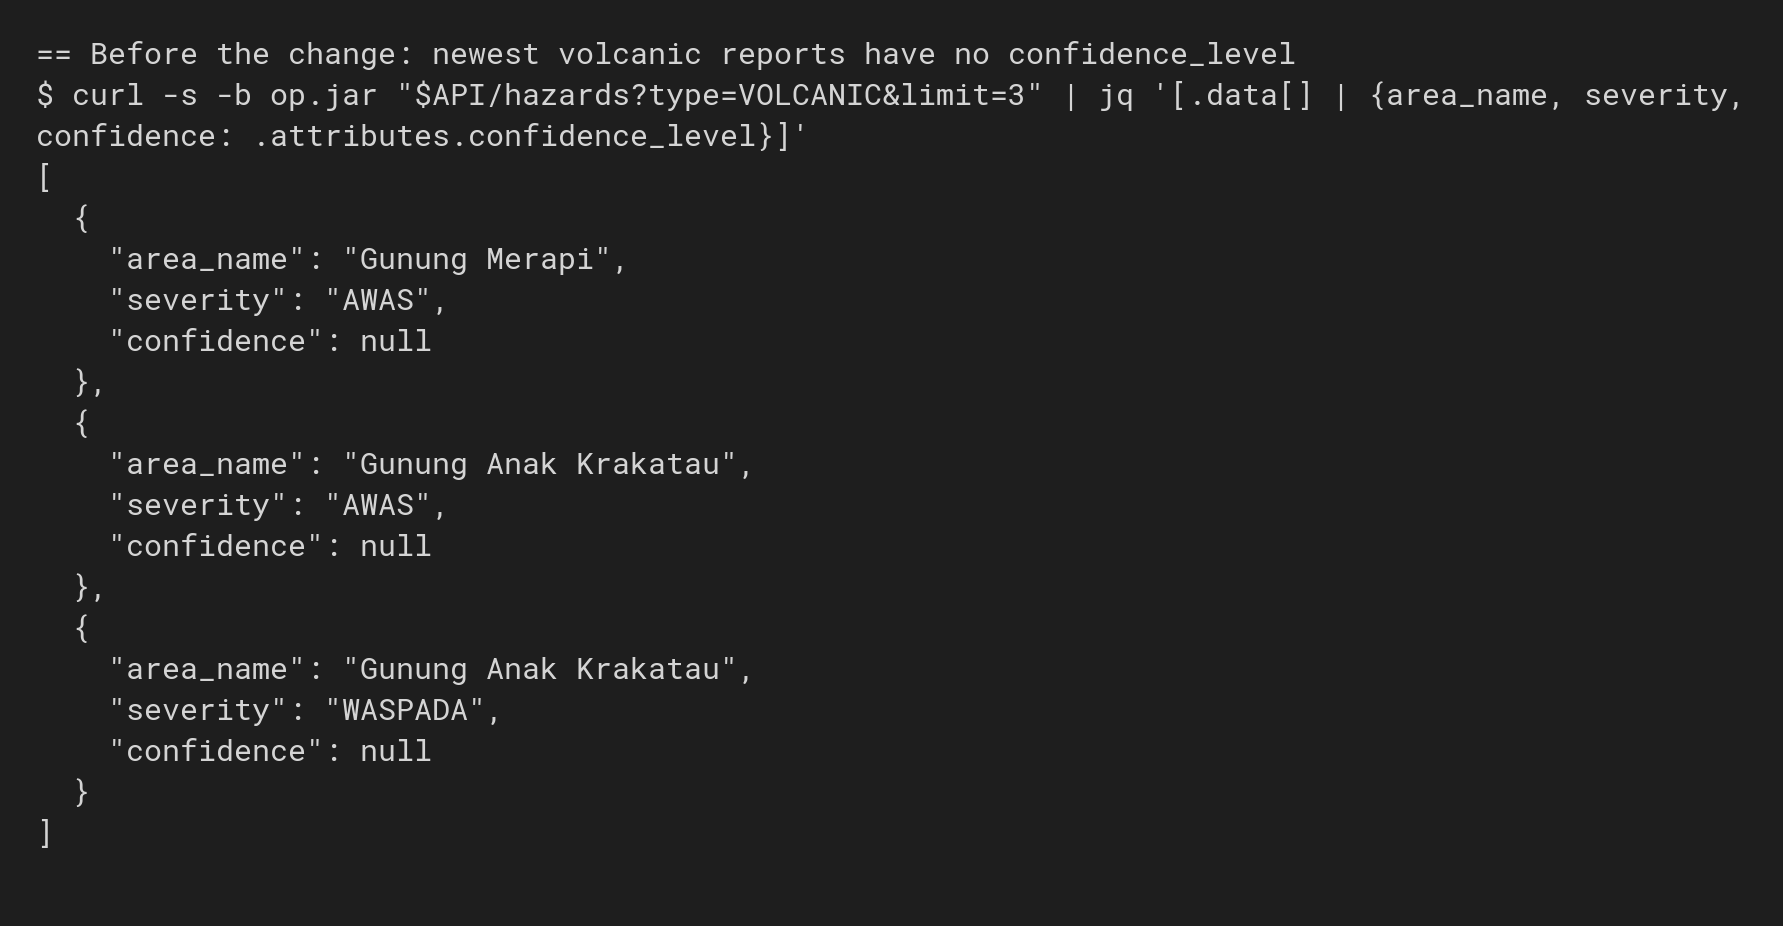
\includegraphics[width=\linewidth,height=0.72\textheight,keepaspectratio]{figures/bukti/vi1.png}
\caption{Tiga laporan vulkanik terbaru sebelum perubahan skema}
\end{figure}

\subsection{Picu Perubahan Skema PVMBG}

Perubahan skema dipicu lewat endpoint admin PVMBG tanpa me-restart mock maupun Aggregator.

\begin{figure}[H]
\centering
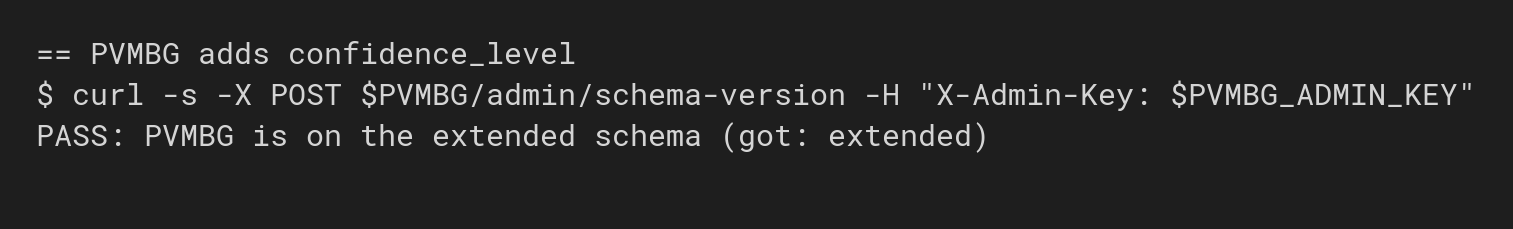
\includegraphics[width=\linewidth,height=0.72\textheight,keepaspectratio]{figures/bukti/vi2.png}
\caption{Memicu perubahan skema PVMBG}
\end{figure}

\subsection{Aggregator Tetap Menghasilkan HazardEvent}

Setelah perubahan, laporan baru membawa \texttt{confidence\_level} di \texttt{attributes}, laporan lama tetap terbaca, dan waktu mulai kontainer Aggregator tidak berubah. Tabel \texttt{hazard\_events} menyimpan rekaman sebelum dan sesudah perubahan berdampingan tanpa migrasi (kolom \texttt{has\_confidence} adalah hasil pemeriksaan \texttt{attributes ? 'confidence\_level'}).

\begin{figure}[H]
\centering
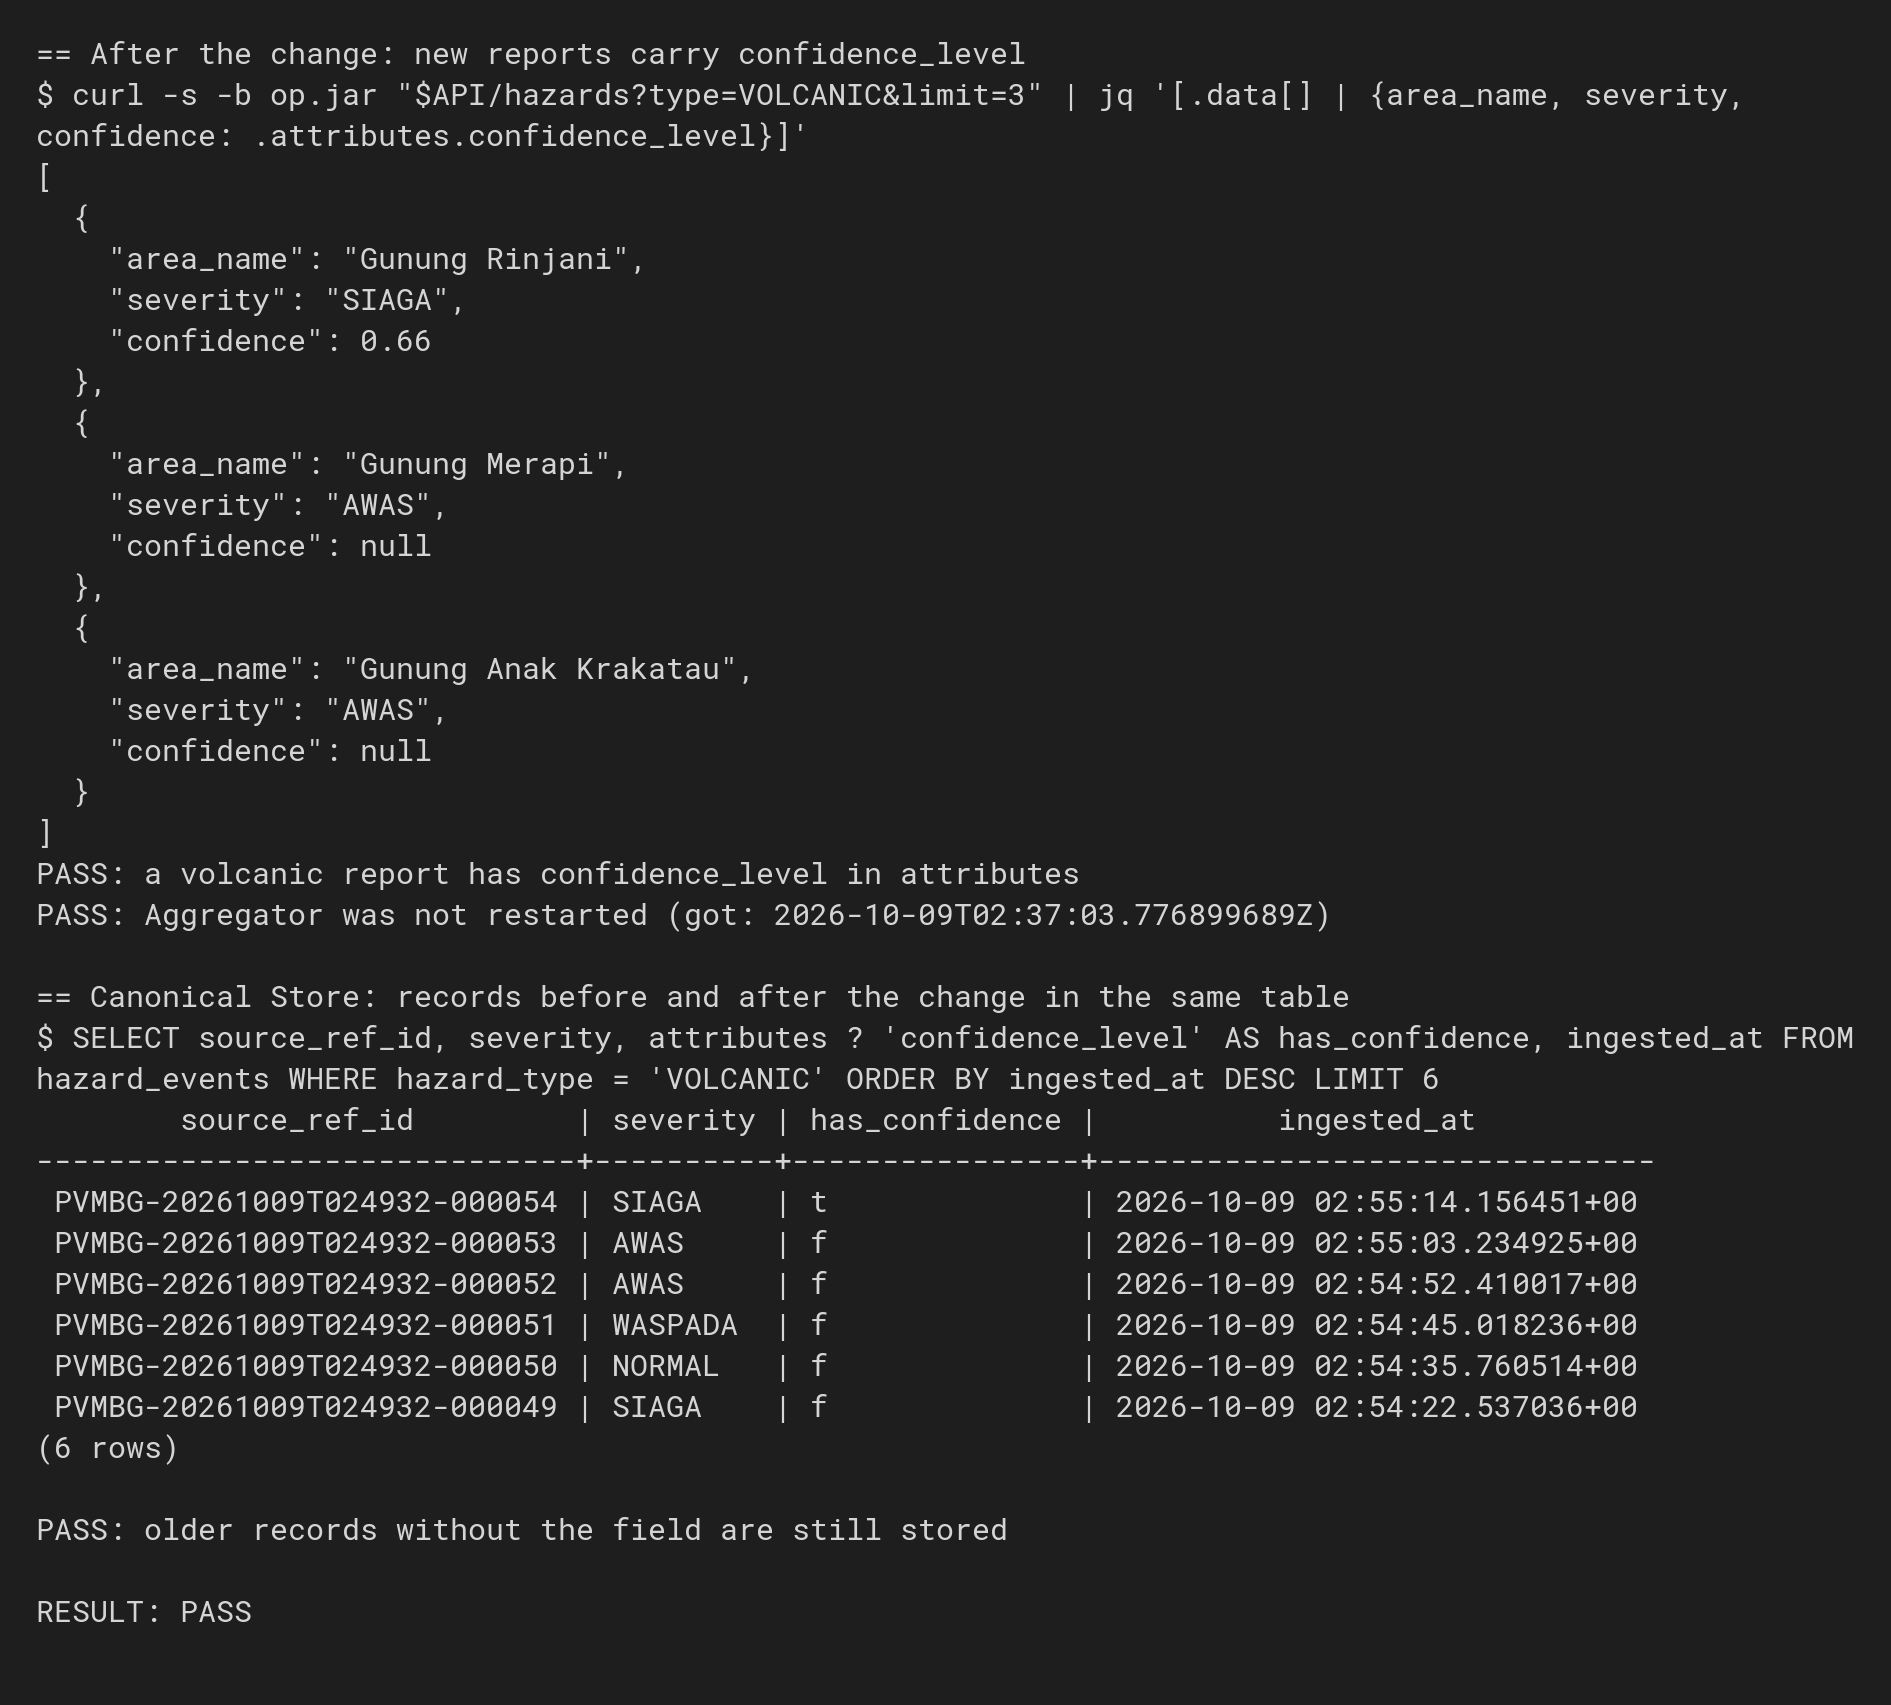
\includegraphics[width=\linewidth,height=0.72\textheight,keepaspectratio]{figures/bukti/vi3.png}
\caption{Laporan sesudah perubahan dan isi tabel \texttt{hazard\_events}}
\end{figure}

